\hypertarget{stm32f4xx__hal__spi_8c}{}\section{Dokumentacja pliku S\+T\+M/\+W\+D\+S\+\_\+\+Kosc\+\_\+\+Linux/\+Drivers/\+S\+T\+M32\+F4xx\+\_\+\+H\+A\+L\+\_\+\+Driver/\+Src/stm32f4xx\+\_\+hal\+\_\+spi.c}
\label{stm32f4xx__hal__spi_8c}\index{S\+T\+M/\+W\+D\+S\+\_\+\+Kosc\+\_\+\+Linux/\+Drivers/\+S\+T\+M32\+F4xx\+\_\+\+H\+A\+L\+\_\+\+Driver/\+Src/stm32f4xx\+\_\+hal\+\_\+spi.\+c@{S\+T\+M/\+W\+D\+S\+\_\+\+Kosc\+\_\+\+Linux/\+Drivers/\+S\+T\+M32\+F4xx\+\_\+\+H\+A\+L\+\_\+\+Driver/\+Src/stm32f4xx\+\_\+hal\+\_\+spi.\+c}}


S\+PI H\+AL module driver. This file provides firmware functions to manage the following functionalities of the Serial Peripheral Interface (S\+PI) peripheral\+:  


{\ttfamily \#include \char`\"{}stm32f4xx\+\_\+hal.\+h\char`\"{}}\newline
Wykres zależności załączania dla stm32f4xx\+\_\+hal\+\_\+spi.\+c\+:\nopagebreak
\begin{figure}[H]
\begin{center}
\leavevmode
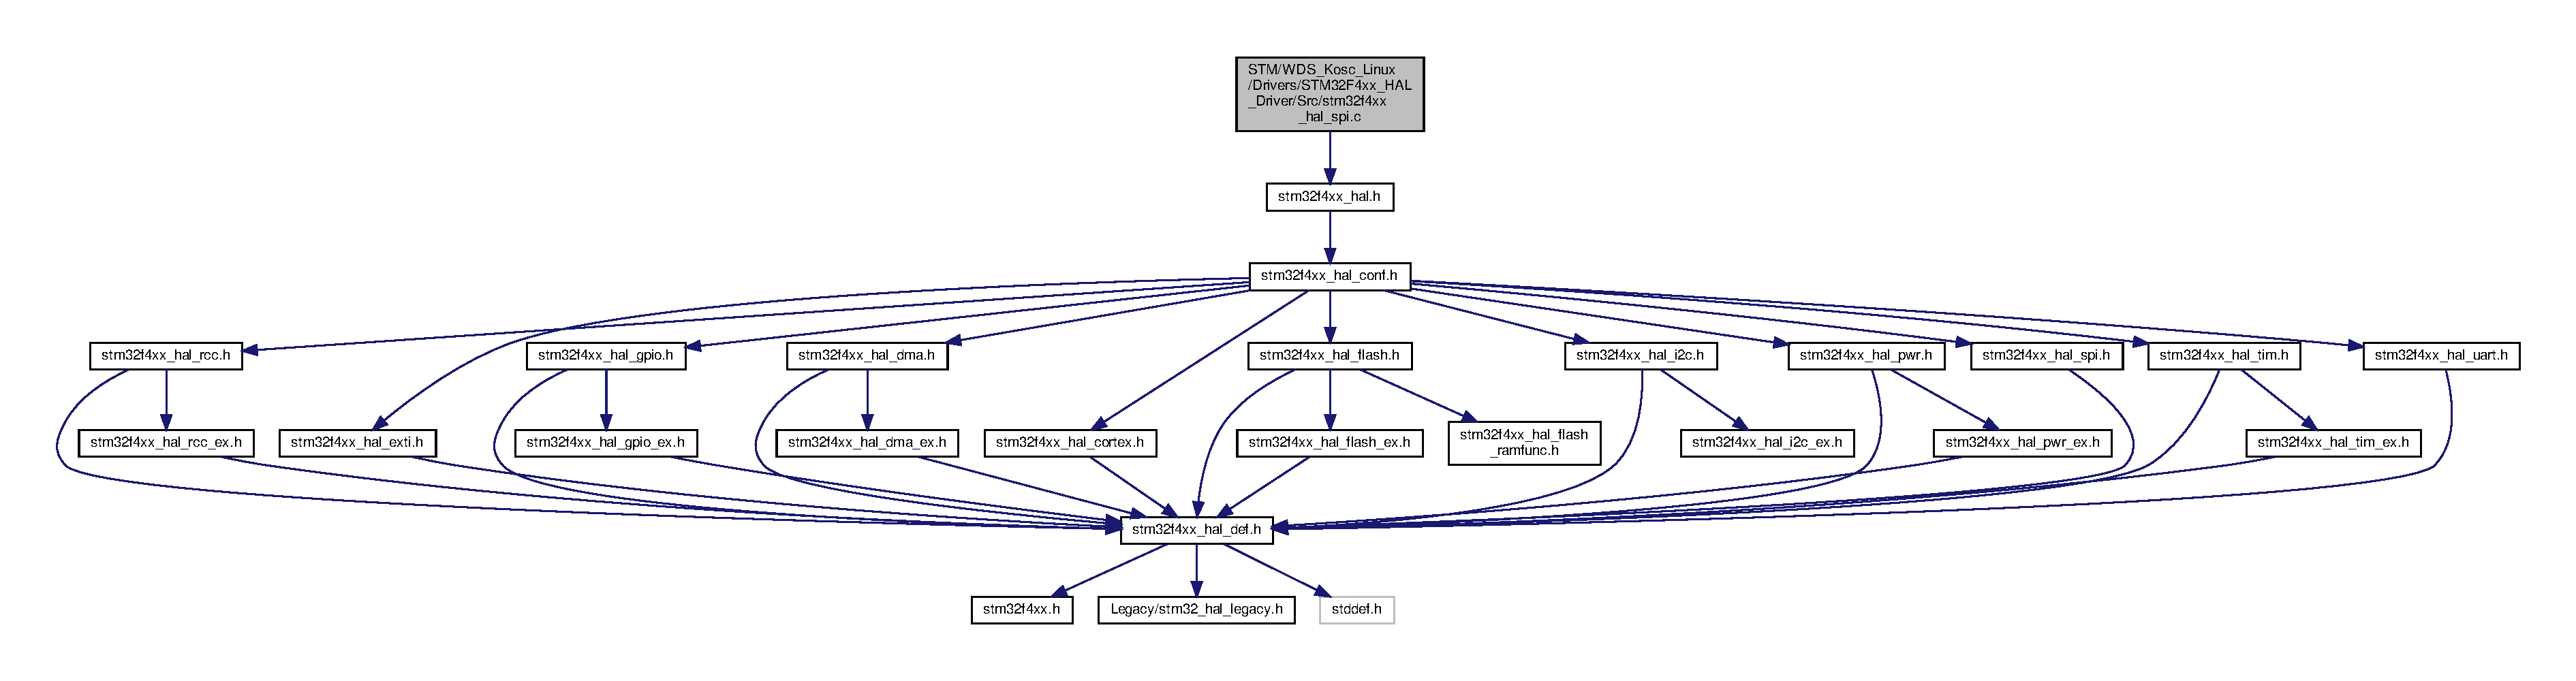
\includegraphics[width=350pt]{stm32f4xx__hal__spi_8c__incl}
\end{center}
\end{figure}


\subsection{Opis szczegółowy}
S\+PI H\+AL module driver. This file provides firmware functions to manage the following functionalities of the Serial Peripheral Interface (S\+PI) peripheral\+: 

\begin{DoxyAuthor}{Autor}
M\+CD Application Team
\begin{DoxyItemize}
\item Initialization and de-\/initialization functions
\item IO operation functions
\item Peripheral Control functions
\item Peripheral State functions
\end{DoxyItemize}
\end{DoxyAuthor}
\begin{DoxyVerb}==============================================================================
                      ##### How to use this driver #####
==============================================================================
  [..]
    The SPI HAL driver can be used as follows:

    (#) Declare a SPI_HandleTypeDef handle structure, for example:
        SPI_HandleTypeDef  hspi;

    (#)Initialize the SPI low level resources by implementing the HAL_SPI_MspInit() API:
        (##) Enable the SPIx interface clock
        (##) SPI pins configuration
            (+++) Enable the clock for the SPI GPIOs
            (+++) Configure these SPI pins as alternate function push-pull
        (##) NVIC configuration if you need to use interrupt process
            (+++) Configure the SPIx interrupt priority
            (+++) Enable the NVIC SPI IRQ handle
        (##) DMA Configuration if you need to use DMA process
            (+++) Declare a DMA_HandleTypeDef handle structure for the transmit or receive Stream/Channel
            (+++) Enable the DMAx clock
            (+++) Configure the DMA handle parameters
            (+++) Configure the DMA Tx or Rx Stream/Channel
            (+++) Associate the initialized hdma_tx(or _rx)  handle to the hspi DMA Tx or Rx handle
            (+++) Configure the priority and enable the NVIC for the transfer complete interrupt on the DMA Tx or Rx Stream/Channel

    (#) Program the Mode, BidirectionalMode , Data size, Baudrate Prescaler, NSS
        management, Clock polarity and phase, FirstBit and CRC configuration in the hspi Init structure.

    (#) Initialize the SPI registers by calling the HAL_SPI_Init() API:
        (++) This API configures also the low level Hardware GPIO, CLOCK, CORTEX...etc)
            by calling the customized HAL_SPI_MspInit() API.
   [..]
     Circular mode restriction:
    (#) The DMA circular mode cannot be used when the SPI is configured in these modes:
        (##) Master 2Lines RxOnly
        (##) Master 1Line Rx
    (#) The CRC feature is not managed when the DMA circular mode is enabled
    (#) When the SPI DMA Pause/Stop features are used, we must use the following APIs
        the HAL_SPI_DMAPause()/ HAL_SPI_DMAStop() only under the SPI callbacks
   [..]
     Master Receive mode restriction:
    (#) In Master unidirectional receive-only mode (MSTR =1, BIDIMODE=0, RXONLY=1) or
        bidirectional receive mode (MSTR=1, BIDIMODE=1, BIDIOE=0), to ensure that the SPI
        does not initiate a new transfer the following procedure has to be respected:
        (##) HAL_SPI_DeInit()
        (##) HAL_SPI_Init()
   [..]
     Callback registration:

    (#) The compilation flag USE_HAL_SPI_REGISTER_CALLBACKS when set to 1U
        allows the user to configure dynamically the driver callbacks.
        Use Functions HAL_SPI_RegisterCallback() to register an interrupt callback.

        Function HAL_SPI_RegisterCallback() allows to register following callbacks:
          (++) TxCpltCallback        : SPI Tx Completed callback
          (++) RxCpltCallback        : SPI Rx Completed callback
          (++) TxRxCpltCallback      : SPI TxRx Completed callback
          (++) TxHalfCpltCallback    : SPI Tx Half Completed callback
          (++) RxHalfCpltCallback    : SPI Rx Half Completed callback
          (++) TxRxHalfCpltCallback  : SPI TxRx Half Completed callback
          (++) ErrorCallback         : SPI Error callback
          (++) AbortCpltCallback     : SPI Abort callback
          (++) MspInitCallback       : SPI Msp Init callback
          (++) MspDeInitCallback     : SPI Msp DeInit callback
        This function takes as parameters the HAL peripheral handle, the Callback ID
        and a pointer to the user callback function.


    (#) Use function HAL_SPI_UnRegisterCallback to reset a callback to the default
        weak function.
        HAL_SPI_UnRegisterCallback takes as parameters the HAL peripheral handle,
        and the Callback ID.
        This function allows to reset following callbacks:
          (++) TxCpltCallback        : SPI Tx Completed callback
          (++) RxCpltCallback        : SPI Rx Completed callback
          (++) TxRxCpltCallback      : SPI TxRx Completed callback
          (++) TxHalfCpltCallback    : SPI Tx Half Completed callback
          (++) RxHalfCpltCallback    : SPI Rx Half Completed callback
          (++) TxRxHalfCpltCallback  : SPI TxRx Half Completed callback
          (++) ErrorCallback         : SPI Error callback
          (++) AbortCpltCallback     : SPI Abort callback
          (++) MspInitCallback       : SPI Msp Init callback
          (++) MspDeInitCallback     : SPI Msp DeInit callback

     [..]
     By default, after the HAL_SPI_Init() and when the state is HAL_SPI_STATE_RESET
     all callbacks are set to the corresponding weak functions:
     examples HAL_SPI_MasterTxCpltCallback(), HAL_SPI_MasterRxCpltCallback().
     Exception done for MspInit and MspDeInit functions that are
     reset to the legacy weak functions in the HAL_SPI_Init()/ HAL_SPI_DeInit() only when
     these callbacks are null (not registered beforehand).
     If MspInit or MspDeInit are not null, the HAL_SPI_Init()/ HAL_SPI_DeInit()
     keep and use the user MspInit/MspDeInit callbacks (registered beforehand) whatever the state.

     [..]
     Callbacks can be registered/unregistered in HAL_SPI_STATE_READY state only.
     Exception done MspInit/MspDeInit functions that can be registered/unregistered
     in HAL_SPI_STATE_READY or HAL_SPI_STATE_RESET state,
     thus registered (user) MspInit/DeInit callbacks can be used during the Init/DeInit.
     Then, the user first registers the MspInit/MspDeInit user callbacks
     using HAL_SPI_RegisterCallback() before calling HAL_SPI_DeInit()
     or HAL_SPI_Init() function.

     [..]
     When the compilation define USE_HAL_PPP_REGISTER_CALLBACKS is set to 0 or
     not defined, the callback registering feature is not available
     and weak (surcharged) callbacks are used.

   [..]
     Using the HAL it is not possible to reach all supported SPI frequency with the different SPI Modes,
     the following table resume the max SPI frequency reached with data size 8bits/16bits,
       according to frequency of the APBx Peripheral Clock (fPCLK) used by the SPI instance.\end{DoxyVerb}


Additional table \+: \begin{DoxyVerb} DataSize = SPI_DATASIZE_8BIT:
 +----------------------------------------------------------------------------------------------+
 |         |                | 2Lines Fullduplex   |     2Lines RxOnly    |         1Line        |
 | Process | Tranfert mode  |---------------------|----------------------|----------------------|
 |         |                |  Master  |  Slave   |  Master   |  Slave   |  Master   |  Slave   |
 |==============================================================================================|
 |    T    |     Polling    | Fpclk/2  | Fpclk/2  |    NA     |    NA    |    NA     |   NA     |
 |    X    |----------------|----------|----------|-----------|----------|-----------|----------|
 |    /    |     Interrupt  | Fpclk/4  | Fpclk/8  |    NA     |    NA    |    NA     |   NA     |
 |    R    |----------------|----------|----------|-----------|----------|-----------|----------|
 |    X    |       DMA      | Fpclk/2  | Fpclk/2  |    NA     |    NA    |    NA     |   NA     |
 |=========|================|==========|==========|===========|==========|===========|==========|
 |         |     Polling    | Fpclk/2  | Fpclk/2  | Fpclk/64  | Fpclk/2  | Fpclk/64  | Fpclk/2  |
 |         |----------------|----------|----------|-----------|----------|-----------|----------|
 |    R    |     Interrupt  | Fpclk/8  | Fpclk/8  | Fpclk/64  | Fpclk/2  | Fpclk/64  | Fpclk/2  |
 |    X    |----------------|----------|----------|-----------|----------|-----------|----------|
 |         |       DMA      | Fpclk/2  | Fpclk/2  | Fpclk/64  | Fpclk/2  | Fpclk/128 | Fpclk/2  |
 |=========|================|==========|==========|===========|==========|===========|==========|
 |         |     Polling    | Fpclk/2  | Fpclk/4  |     NA    |    NA    | Fpclk/2   | Fpclk/64 |
 |         |----------------|----------|----------|-----------|----------|-----------|----------|
 |    T    |     Interrupt  | Fpclk/2  | Fpclk/4  |     NA    |    NA    | Fpclk/2   | Fpclk/64 |
 |    X    |----------------|----------|----------|-----------|----------|-----------|----------|
 |         |       DMA      | Fpclk/2  | Fpclk/2  |     NA    |    NA    | Fpclk/2   | Fpclk/128|
 +----------------------------------------------------------------------------------------------+

 DataSize = SPI_DATASIZE_16BIT:
 +----------------------------------------------------------------------------------------------+
 |         |                | 2Lines Fullduplex   |     2Lines RxOnly    |         1Line        |
 | Process | Tranfert mode  |---------------------|----------------------|----------------------|
 |         |                |  Master  |  Slave   |  Master   |  Slave   |  Master   |  Slave   |
 |==============================================================================================|
 |    T    |     Polling    | Fpclk/2  | Fpclk/2  |    NA     |    NA    |    NA     |   NA     |
 |    X    |----------------|----------|----------|-----------|----------|-----------|----------|
 |    /    |     Interrupt  | Fpclk/4  | Fpclk/4  |    NA     |    NA    |    NA     |   NA     |
 |    R    |----------------|----------|----------|-----------|----------|-----------|----------|
 |    X    |       DMA      | Fpclk/2  | Fpclk/2  |    NA     |    NA    |    NA     |   NA     |
 |=========|================|==========|==========|===========|==========|===========|==========|
 |         |     Polling    | Fpclk/2  | Fpclk/2  | Fpclk/64  | Fpclk/2  | Fpclk/32  | Fpclk/2  |
 |         |----------------|----------|----------|-----------|----------|-----------|----------|
 |    R    |     Interrupt  | Fpclk/4  | Fpclk/4  | Fpclk/64  | Fpclk/2  | Fpclk/64  | Fpclk/2  |
 |    X    |----------------|----------|----------|-----------|----------|-----------|----------|
 |         |       DMA      | Fpclk/2  | Fpclk/2  | Fpclk/64  | Fpclk/2  | Fpclk/128 | Fpclk/2  |
 |=========|================|==========|==========|===========|==========|===========|==========|
 |         |     Polling    | Fpclk/2  | Fpclk/2  |     NA    |    NA    | Fpclk/2   | Fpclk/32 |
 |         |----------------|----------|----------|-----------|----------|-----------|----------|
 |    T    |     Interrupt  | Fpclk/2  | Fpclk/2  |     NA    |    NA    | Fpclk/2   | Fpclk/64 |
 |    X    |----------------|----------|----------|-----------|----------|-----------|----------|
 |         |       DMA      | Fpclk/2  | Fpclk/2  |     NA    |    NA    | Fpclk/2   | Fpclk/128|
 +----------------------------------------------------------------------------------------------+
 @note The max SPI frequency depend on SPI data size (8bits, 16bits),
       SPI mode(2 Lines fullduplex, 2 lines RxOnly, 1 line TX/RX) and Process mode (Polling, IT, DMA).
 @note
      (#) TX/RX processes are HAL_SPI_TransmitReceive(), HAL_SPI_TransmitReceive_IT() and HAL_SPI_TransmitReceive_DMA()
      (#) RX processes are HAL_SPI_Receive(), HAL_SPI_Receive_IT() and HAL_SPI_Receive_DMA()
      (#) TX processes are HAL_SPI_Transmit(), HAL_SPI_Transmit_IT() and HAL_SPI_Transmit_DMA()
\end{DoxyVerb}


\begin{DoxyAttention}{Uwaga}

\end{DoxyAttention}
\subsubsection*{\begin{center}\copyright{} Copyright (c) 2016 S\+T\+Microelectronics. All rights reserved.\end{center} }

This software component is licensed by ST under B\+SD 3-\/\+Clause license, the \char`\"{}\+License\char`\"{}; You may not use this file except in compliance with the License. You may obtain a copy of the License at\+: opensource.\+org/licenses/\+B\+S\+D-\/3-\/\+Clause 